\chapter{Introduction} \label{s:introduction:introduction}

Computer networks have become the predominant communications media of the
digital era. Nonetheless, the widening adoption of network technologies has
highlighted several scalability problems in network functionality. These
primarily derive from the design of network protocols and architectures.
Addressing these limitations through protocol redesign is a challenging process,
which requires significant time and effort for deployment. Network systems
require novel backwards-compatible mechanisms that provide scalable performance. 

This dissertation is concerned with performance scalability problems in modern
networks.  The thesis of this dissertation is that control plane redesign can
mitigate network bottlenecks, introduced by protocol design, while ensuring
backwards compatibility and high performance. We argue that existing control
plane mechanisms remain inflexible and that their ``single abstraction fits all''
approach fails to fulfil the unique requirements of a set of novel deployment
environments, e.g.~datacenters and home networks.  We advocate that
networks require control redesign, \textit{tailored} to the requirement and
opportunities of  the environment. The recent rebirth of SDN in network devices
provides a sufficient and readily-available enabler for the proposed approach. 
% In order to achieve this, we propose the
% incorporation of the SDN paradigm as our technology enabler. 
% \todo{there is a strong requirement for refinement here.}

For the remainder of this chapter, we discuss the motivations of our work
(\S~\ref{sec:intro:motivations}), followed by the explicit definition of our
contributions (\S~\ref{sec:intro:contributions}) and  the outline of this thesis
(\S~\ref{sec:intro:outline}).

% In 2011, a third of the global population is Internet-connected through a wide
% range of network technologies~\mycite{itufacts2011}, while Internet resources,
% based on estimations, generate 3.4\% of the global GDP~\mycite{duRausas:2011un}.

% Due to the increasing importance of network technologies, functional
% requirements are constantly evolving and network infrastructures {\emph must} be
% future-proof against increasing traffic rates and performance and security
% policy complexity.

\section{Motivation} \label{sec:intro:motivations}

This section presents the motivations for our thesis. Specifically, motivated by
the radical evolution of current network
technologies(\S~\ref{sec:intro:net_evolution}), we discuss the resulting network
performance complexity~(\S~\ref{sec:intro:perf_complexity}) and exemplify some
of the limitation incurred by the design of Internet
protocols~(\S~\ref{sec:intro:control_limitations}).

\subsection{Computer Network Evolution}\label{sec:intro:net_evolution}

% a historical perspective on computer networks 
One of the key mechanisms that formed the objective conditions for the digital
revolution of our era was the concept of packet-switched computer networking.
Computer networks provide a generic data-exchange mechanism between 2 computers
over a physical medium.  The most successful attempt to define and implement a
heterogeneous computer network of significant size was
\textit{ARPANET}~\mycite{beranek81}. ARPANET improved the resilience and
performance of available circuit-switched networks, and its simple design
allowed easy adoption by existing computing systems.  It was adopted by a small
number of US education and research institutes and allowed, for the first time
in computing history, for the interconnection of multiple mainframes using a
packet-switched network. The ARPANET community standardized a small set of
data-exchange protocols, namely: e-mail~\mycite{RFC0561}, FTP~\mycite{RFC0354}
and voice~\mycite{RFC0741}. ARPANET was later replaced by the
NSFNET~\mycite{Mills:1987tt}, which eventually evolved in today's Internet.  As
part of this transition, the research community developed the standards for the
Internet protocol suite~\mycite{Clark:1988,RFC793,RFC1122,RFC0791,RFC894}, the
lower and middle layers of the network stack.

Computer networks, conceived only 20 years after the implementation of a
programmable computer, have gained a significant position in our society since
the ARPANET years, co-evolving with the digital revolution.  Their
communication abstraction replaces a number of traditional communication
systems, while providing support for a wide range of applications and
deployment environments (e.g.~telephone networks).  As a result, in 2011 a
third of the global population is Internet-connected through a wide range of
network technologies~\mycite{itufacts2011}.  The average user is
Internet-connected in parallel through multiple devices (e.g.~laptop,
smartphone, home entertainment system) and a large portion of daily activities
rely on network technologies (e.g.~e-banking, e-gov, online social networking).
The importance of computer networks is further reflected in its importance to
the global economy. Internet resources are estimated to generate 3.4\% of
global GDP~\mycite{duRausas:2011un}, while increasing availability of broadband
connectivity in developing economies exhibits a positive correlation with GDP
growth (10\% increase in the number of households connected to broadband
services improves GDP by approximately 1\%~\mycite{katz2011}).  The growth in
network adoption introduces novel performance requirements for network
technologies and protocols.  

\subsection{The Lernaean Hydra of Network Performance} \label{sec:intro:perf_complexity}

Traditional computer network theory textbooks (such as \mycite{peterson2011})
define network performance using elementary metrics, like latency, bandwidth,
jitter and packet loss. Nevertheless, the increased adoption of network
technologies creates an equal augmentation in network use-cases, and the
definition of performance must preclude the end-user and application
perspective.  Consequently, the definition of network performance becomes
complex and is domain and application-specific, considering additional
subjective aspects like usability.  We elaborate on the complexity and
multidimensionality of performance by discussing two example aspects:
application resource requirements and network heterogeneity. 

\begin{table} 
  \centering 
    \begin{tabular}{| p{5cm} | p{1.8cm} p{1.8cm} p{1cm} p{2.3cm} |} 
      \hline
      Application                                & Throughput (Mbps) & Latency (sec) & Jitter (sec)  & Flow Number (median) \\ \hline
      Web~\mycite{Akamai_4_seconds,Butkiewicz11} & -                 & 4            & -              & 10               \\
      Video~\mycite{Finamore11}                  & 0.3 - 5           & -            & -              & 1                \\
      Peer-to-peer~\mycite{Rasti07,pouwelse2004} & -                 & -            & -              & 30               \\ 
      VoIP                                       & 0.1 - 1.5         & 0.5          & 0.1            & 1                 \\ 
      Gaming~\mycite{armitage2006networking}     & 0.1               & 0.1          & 0.05           & 1                 \\
      \hline 
    \end{tabular} 
  \caption{Network performance requirements for a set of popular traffic classes.} \label{tbl:application_requirement} 
\end{table}

% \todo{tail at
%   scale, add requirements for cloud service providers for map reduced
%  applications.}. 
The availability of the network abstraction in multiple devices and contexts
motivates the development of a wide range of network applications, with global
audiences and diverse performance requirements.  As an example,
Table~\ref{tbl:application_requirement} presents the network requirements in
terms of bandwidth, latency, jitter and number of concurrent flows for web,
video streaming, peer-to-peer,  VoIP and gaming application classes.  Based on
the table, it is evident that current network applications have contradicting
requirements. For example, peer-to-peer applications do not have any
performance requirements but try aggressively to maximize network throughput,
affecting applications with strict latency requirements, like VoIP\@.  As a
result, applications face difficulties in sharing network resources during
times of congestion. Network operators overcome the sharing problem by
over-provisioning bandwidth resources, but physical limitations reduce the
effectiveness of the approach. 

\begin{figure}[] 
  \subfigure[Fixed Internet]
    {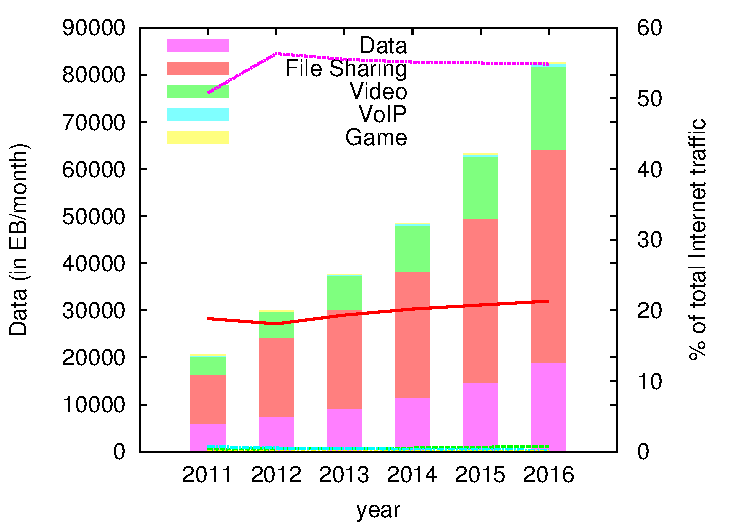
\includegraphics[width=0.49\textwidth]{Introduction/IntroductionFigs/internet}\label{fig:mobile}}  
  \subfigure[Mobile Internet]
  {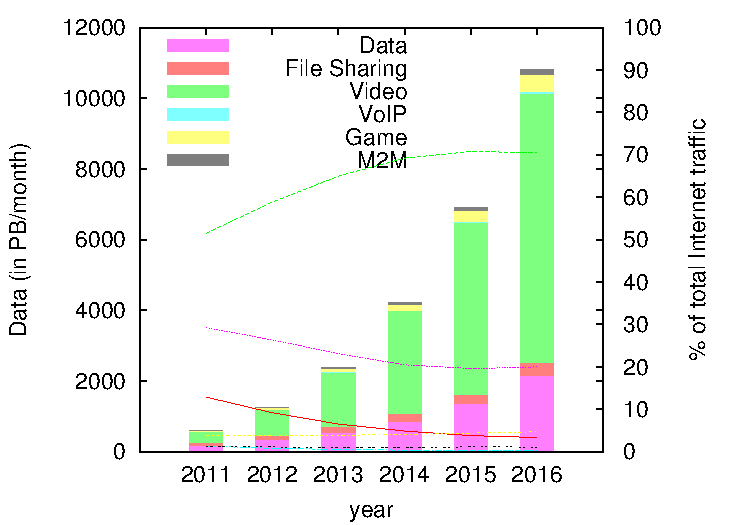
\includegraphics[width=0.49\textwidth]{Introduction/IntroductionFigs/mobile}\label{fig:internet}}
  \caption[Cisco Visual Network Index report on global traffic trends]{Cisco
    Visual Network Index report on global traffic trends
    for fixed (Figure~\ref{fig:internet}) and mobile Internet (Figure~\ref{fig:mobile}).}
  \label{fig:internet_applications} 
\end{figure}

Application performance exhibits similar complexity at a macroscopic level.
Figure~\ref{fig:internet_applications} presents estimated traffic volumes for
six popular network application classes between the years 2011 and 2016 for mobile
and fixed Internet, using data from the Cisco visualization
index~\mycite{Mobile:2012vd,Cisco:2012wu}. Aggregate network traffic volumes
exhibit an exponential augmentation and is expected to increase by an order of
magnitude for mobile Internet, and by four times for fixed Internet between the
years 2011 and 2016. Traffic volume increase is primarily driven by video
delivery applications, which are increasing in popularity over file-sharing
applications. The popularity churn reflects the availability of predominant
file-sharing video content by high-availability CDN services like YouTube.
Even so, the two classes exhibit different characteristics with respect to
bandwidth requirements and network providers are obliged to reflect these
trends in their network architecture and configuration. Furthermore,
application traffic volumes commonly exhibit long-term popularity fluctuation,
but a minimum traffic volume will always exist in the network and shape ISP
policies and architectures. 

% % How does the network look like in terms of point to point connectivity. 
A significant evolution also exists in the lower layers of the network.
Ethernet has been the predominant Internet link layer protocol since the 80's,
mainly due to its low cost and complexity. The network community has defined
standards to implement the Ethernet abstraction over a wide range of medium
types, like copper, fibre, off-licence radio frequencies, satellite links and
GSM networks, encapsulating significant heterogeneity. This approach hides a
number of medium properties (e.g.~link layer ARQ, link rate), which reflect
significant performance characteristics of the link layer. At the same time,
applications, network layer protocols and users remain unaware of these factors
and require homogeneous performance semantics. 

\subsection{Performance Limitations}\label{sec:intro:control_limitations}

Current network protocols have a number of design limitations, primarily
due to the inability to predict the radical adoption of the technology during
their development.  The early adopters of the NSFNET, the incubator  of
Internet protocol standards, were universities and research facilities, and the
resulting system aimed to support asynchronous communication, low data-rates,
open service connectivity and best-effort guarantees. These initial assumptions
have been radically revised in the Internet over the years, but the protocol
designs have not managed to keep up with their evolution. The mismatch between
protocol capabilities and current requirements grows in proportion to the
increase of link speeds.
% ~\todo{ratio of transmission to propagation delay is reduced}.  

In parallel, the evolution of network technologies, and especially of their
control plane, has highlighted that the adopters dictate that abstraction
simplicity as a primary design goal. The Internet protocol definition process
followed a Darwinian selection approach between available solutions during the
early days of NSFNET\@. Along with the TCP/IP protocol suite, OSI and ITU
proposed equivalent protocol stacks~\mycite{x.213,x.233}, while the ATM Forum
also defined similar higher-layer protocols~\mycite{Siu95}. These protocol
design efforts defined detailed abstractions which addressed some current
functional limitations.  For example, ATM provided strong resource guarantees,
motivated by the fixed cell size and circuit-based forwarding approach.
Nonetheless, their high complexity faces performance scalability problems with
respect to available computational resources, and the protocols became obsolete
in favour of the TCP/IP protocol suite. For the rest of the section we will
discuss in detail some examples of network bottlenecks, which have arisen as a
consequence of the design of current network protocols.

% \subparagraph*{Security} 
% 
% The initial security requirements for computer network technologies were
% minimal. On one hand, early technology adopters, such as educational and
% research institutes, used networks to provide open, free and accessible
% services, aiming to augment technology adoption. As a result, their security
% requirements were minimal. On the other hand, the computing resources of the
% time were limited and couldn't support the computation requirements for a
% security-aware network design.  In parallel the US Department of Defence~(DoD) ,
% in order to ensure secure transmission of classified information, designed and
% implemented a number of high security networks, namely MILNET, SIPRnet and
% NIPRnet. These networks function as partially stand-alone inter-networks owned
% by the DoD and provide strong security primitives in the network design.  Their
% design supports low bandwidth connectivity~(primarily HTTP and mail services)
% and uses enhanced security mechanisms in the lower layers of the stack along
% with existing Internet protocol in the higher layers of the
% network~\mycite{siprnet}. 
% 
% These initial network security requirements are currently invalidated. A McAfee
% report from 2009 estimates the cost for cybersecurity to approximately 600
% million dollars~\mycite{kanan2009unsecured}.  Similarly, during the wikileaks
% scandal in 2011~\mycite{cablegate}, a significant number of US state documents was
% intercepted from the SIPRnet system, exposing the limitation in the design of
% the network.  The threat model for network systems is wide and contains numerous
% attacks; from information interception to denial-of-service attacks.  The
% research community has proposed a number of protocols to address the security
% requirements of today network environment, e.g.~IPSEC~\mycite{RFC2401} and loose
% source routing~\mycite{Argyraki09}.  Nonetheless, although such protocol introduce
% enhanced security guarantees for the data plane, they also introduce significant
% complexity on the control plane of the network. For example, for IPsec the data
% plane can implement at line rate the encryption/decryption task, but an IPsec
% gateway must maintain protocol state for each tunnel.  Network security requires
% security-aware control logic spanning from the lowest layers of the network
% abstraction and spread across the network. 

% \subparagraph*{Network Addressing} When the IP protocol was firstly deployed
% in the Internet, the size of the network was sufficiently small. Host
% addresses use a 32-bit integer, split in byte aligned classes in order to
% permit aggregation at the forwarding entities. Within 10 years, the initial
% assumptions over the size of classes was re-established through the classless
% Inter-domain routing (CIDR), in order to allow better utilisation of the IP
% space. Within 15 years the initial assumption over the size of the address
% space proved also short-sighted, as IP addresses were not sufficient to cover
% the needs of hosts.  A number of layer violations, like NATs, were widely used
% within the subsequent years in order to provide connectivity to the increasing
% number of end-hosts. In order to address this problem within the design of the
% network protocol, a revised version of IP has been proposed~\mycite{RFC2460}
% since 1998, but its deployment is slow, as the size of the current Internet
% makes it extremely difficult to replace IPv4 without significant connectivity
% problems and costs.

\subparagraph{Network management scalability}

Policy and configuration interfaces in current networks introduce a significant
performance bottleneck.  \mycite{Mahajan02} pinpoint a significant portion of
global BGP routing errors to protocol misconfigurations, prompted to a great
extent by the counter-intuitive configuration interface.  \mycite{Kim11} study
the configuration evolution of two medium-sized campus networks and highlight
the limitations of current configuration interfaces.  Device configuration
files exhibit a continual size increase, containing frequently stale rules that
are pruned only during policy conflicts or major policy revisions.  Interfaces
remain low-level and inexpressive. As a result, network policy updates
translate into multiple device reconfigurations, while forwarding and security
policies are merged by the device interface. The configuration bottleneck is
equally important in environments with non-expert administrators, like the home
network. \mycite{grinter05} conclude that the human understanding of network
abstraction is limited and the complexity of control abstraction leads to
under-optimized network configurations, especially  in terms of security and
performance. 

Currently, network configuration relies to a great extent on the network
administrator, who is responsible for manually transforming the network policy into
specialised configurations for each network device and network layer.  For
example, the policy must be translated both into VLAN tagging configurations in
the data-link layer, and routing and firewall configurations for the network
layer.  Section~\ref{sec:background:forwarding} provides an extensive
presentation of current network control mechanisms and available control
abstractions.  The rapid development of network technologies has limited
effect on device interfaces, which remain low-level and counter-intuitive to
administrators. As a result, network configuration still remains a process
requiring and relying on the experience of the network administrator.  Effectively,
network management interfaces introduce a bottleneck on the ``mechanism''
translating the network policy into distributed device configurations the
network administrator.  

Network management requires a technological ``revolution'', similar to the
introduction of high-level programming languages in the 70's.  In order to
scale network management performance, we require new, user-friendly control
abstractions, which can automate the process of policy translation, unify the
control domain across the network and specialize the control plane
functionality to the deployment environment. 

\subparagraph*{Resource allocation} 

As discussed in Section~\ref{sec:intro:perf_complexity}, modern network
functionality requires dynamic, fine grain and rapid resource control in order
to fulfil the diverse application requirements.  Network engineers commonly
address this problem through resource over-provision~\mycite{TeiSha02}, which,
however, produces reduced effectiveness at high link-rates. High access speeds
increase application responsiveness and similarly shape end-user
expectations.  Although, during high link utilisation incidents, network
responsiveness and user experience degrade severely, in the vicinity of
queueing delays and packet losses.  A number of mechanisms have been proposed to
improve resource control, in various layers of the network stack
(e.g.~ECN~\mycite{RFC5562}, DiffServ~\mycite{RFC2475}, RSVP over
MPLS-TE~\mycite{RFC3209}). These mechanisms however, for different reasons,  fail to
provide a generic solution to the problem. 

The ideal mechanism for effective resource control requires a priori knowledge
of resource requirements from end-hosts in order to define optimal resource
allocations.  Currently, networks follow a distributed approximation using a
feedback mechanism between two systems: the end-to-end congestion control; and
the network forwarding policy.  End-to-end congestion control infers the
available bandwidth of the network path using flow properties, like packet loss
and RTT variance, and adjusts the traffic rate accordingly. The network
forwarding policy defines, statically or dynamically, network paths between
hosts, as well as prioritisation and buffer size for specific network flows.
Forwarding policy decisions can modify flow properties, affect end-to-end
congestion control and enforce resource control policies effectively.
Nonetheless, because the two mechanisms are weakly integrated, policy
enforcement is effective in long timescales.  Resource management in current
networks requires smarter control planes, which augment the inputs to the
decision algorithm and provide faster responses.

\subparagraph*{Connectivity scalability} 

A popular approach to address network scalability problems uses middleboxes;
transparent network devices which redefine the behaviour of data plane
protocols, like NAT boxes, WAN optimizers and firewalls.  Middleboxes have,
 to a great extend, redefined overall protocol functionality, as they commonly
introduce new assumptions into the protocol functionality and violate the
``Robustness principle'' of networks\footnote{``In general, an implementation must
be conservative in its sending behavior, and liberal in its receiving behavior.
That is, it must be careful to send well-formed datagrams, but must accept any
datagram that it can interpret (e.g., not object to technical errors where the
meaning is still clear).''~\mycite{RFC0791}}. In addition, their functionality
and behaviour varies significantly between vendors, and remains inflexible and
isolated from the control plane of the operating network. \mycite{Honda:2011ci}
present an Internet-wide robustness measurement study and report that obscure
but semantically correct protocol behaviours are unsupported by a number of
edge networks, primarily due to the functionality of such devices.
Similarly,~\mycite{Hatonen10} study the operational semantics of a series of
home network routers and highlight significant differences between commercial NAT
implementations. 

A significant side-effect of middlebox functionality is the redefinition of
elementary network properties, like the bi-directionality of network
connectivity.  For example, NAT boxes improve address scalability, but reduce
host reachability.  All hosts behind a NAT are able to access any Internet
service using a single IP address, but require network reconfiguration to expose
an Internet-wide service. A series of protocols has been proposed to 
enable end-hosts middlebox control~\mycite{RFC3234}, but their generality is
limited and context-specific.


% Nonetheless, in order to enable adaptability of network technologies in new
% domains, without loosing the ability to evolve existing protocols, we need to
% integrate middlebox control with the control plane of the network. 


\section{Contributions}\label{sec:intro:contributions}

This dissertation contends that existing network architectures cause a
significant performance bottleneck in network functionality and provide limited
support to the constantly evolving network requirements of end-users.  Modern
networks require flexible and specialized control approaches that address
complex functional requirements, and unify network control across all devices
of the network. Our study employs the SDN control approach and the \of protocol
extensively.  Nonetheless, the applicability of our contributions are not
limited to the \of protocol and can easily adapt to alternative programmable
control frameworks. In detail, we claim the following specific contributions:

\begin{itemize}
  \item \textbf{Control plane scalability}: We provide an in-depth study of SDN
  control scalability. In this context, we present two measurement and
  evaluation platforms for SDN control: \oflops; and \sdnsim. \oflops is a high
  precision switch evaluation platform, providing a range of testing modules
  for elementary \of interaction. \sdnsim is a network experimentation
  platform, specialised for \of control architectures, which allows a user to
  easily describe and either simulate or emulate an experimental setup. These
  two platforms establish a generic toolbox, providing a flexible evaluation of
  SDN control applications. Using these tools, we provide an in-depth analysis
  of control plane performance and limitations for a  wide range of
  off-the-self \of implementations. Additionally, using as an input the
  \oflops performance models, we explore the impact of a hierarchical
  control  scheme on the performance of a small-scale datacenter. 
 
  \item \textbf{Network management scalability}: We present a control
  application which addresses the problem of network management and resource
  control. We consider the multiple and varied domain of the home network.
  Motivated by recent ethnographic and measurement studies for home networks,
  we identify user requirements for accurate network state information and
  intuitive control primitives. We address these requirement through the home
  router, by redesigning the control plane functionality.  While maintaining
  full compatibility with existing network applications, our design provides a
  user intuitive control abstraction, which incorporates the user's social
  input into the forwarding decision and improves both access control and QoS.

  \item \textbf{Naming and Connectivity scalability}: We revisit the problem of
  connectivity scalability in the Internet.  Our exploration is motivated by
  the requirement of end-users to interconnect devices across the Internet in
  an ad hoc manner, thus forming Personal Clouds. Currently, this requirement
  is fulfilled through data offloading to third party cloud services, raising
  concerns regarding performance, efficiency and security.  We propose
  \signpost, a distributed control plane architecture for end-hosts, which
  provides inter-device connectivity and controllable performance and security
  across the network. In addition, simple augmentation of end-host forwarding
  logic, allows \signpost to integrate seamlessly with a wide range of existing
  resource sharing applications.
\end{itemize}

\section{Outline} \label{sec:intro:outline}

The rest of this dissertation is organised as follows.
Chapter~\ref{ch:background} provides background information related to our
thesis. Motivated by the architecture of current network devices and the
physical and design limitation of network control, we revisit control plane
mechanisms and related research efforts into control plane scalability.  

In Chapter~\ref{sec:sdn_scalability} we study the control scalability of the
SDN paradigm.  We present two control plane benchmarking platforms,
\textit{OFLOPS} and \textit{SDNSIM}, designed to provide high precision
evaluation of the scalability of \of{} devices and architectures, respectively.
Using these tools, we conduct a measurement study to characterise the
performance of baseline \of{} operation by SDN-enabled devices and the impact
of distributed control architectures in the data plane performance.  In
Chapter~\ref{sec:homework}, we study the problem of control plane management
performance, focusing on the home network setting. Using existing user studies,
we draw out the user network management requirements and redesign the control plane
architecture of the home router. Our architecture provides a simpler,
user-friendly control abstraction which fulfils the user requirements for
control and information from their network. In addition, we provide an
extensive evaluation of the architecture, providing evidence on scalability
and backwards compatibility.  In Chapter~\ref{sec:signpost} we investigate
the application of the SDN paradigm in naming and connectivity scalability to
create a federated network between a user's devices. We present \signpost,
a novel user-centric control plane architecture, providing Internet-wide device
connectivity with user-controlled performance and security. We also present the
architecture of the framework, its integration with existing
connectivity-enabling mechanisms and we evaluate the performance and
applicability of the framework.  Finally, in Chapter~\ref{sec:conclusions} we
draw conclusions from our study and discuss areas for further study. 
